\section{Microprocessor}

A microprocessor is a general-purpose processor responsible for running embedded applications.
Microcontrollers form the core of many modern, pervasive computing applications. 
These tiny, cost-effective computers are designed for specific tasks, making them ideal for embedded systems.

Unlike traditional computers, microcontrollers do not require an operating system. 
Instead, they run firmware (software that is directly executed on the hardware). 
This firmware includes low-level instructions to manage peripherals and system functions.
The defining feature of microcontrollers is that they integrate all essential components into a single silicon chip.

\subsection{Microcontroller}
Microcontrollers have a fixed hardware architecture built around a central processing unit. 
The CPU manages a range of peripherals, providing both digital and analog functionality.
Smaller devices typically include both volatile (RAM) and non-volatile (flash) memory on the chip, while more powerful processors may require external memory.
Programming is commonly done using low-level languages like Assembly or high-level languages like C.

Microcontrollers are the preferred choice for embedded systems because they integrate essential components like memory and peripherals, reducing the need for additional circuitry. 
This allows for compact, power-efficient designs that are crucial in space-constrained applications.
A microcontroller typically consists of a microprocessor with program (flash) and data (RAM) memory and various on-chip peripherals.
Modern microcontrollers have significantly improved in both performance and efficiency. 

\begin{figure}[H]
    \centering
    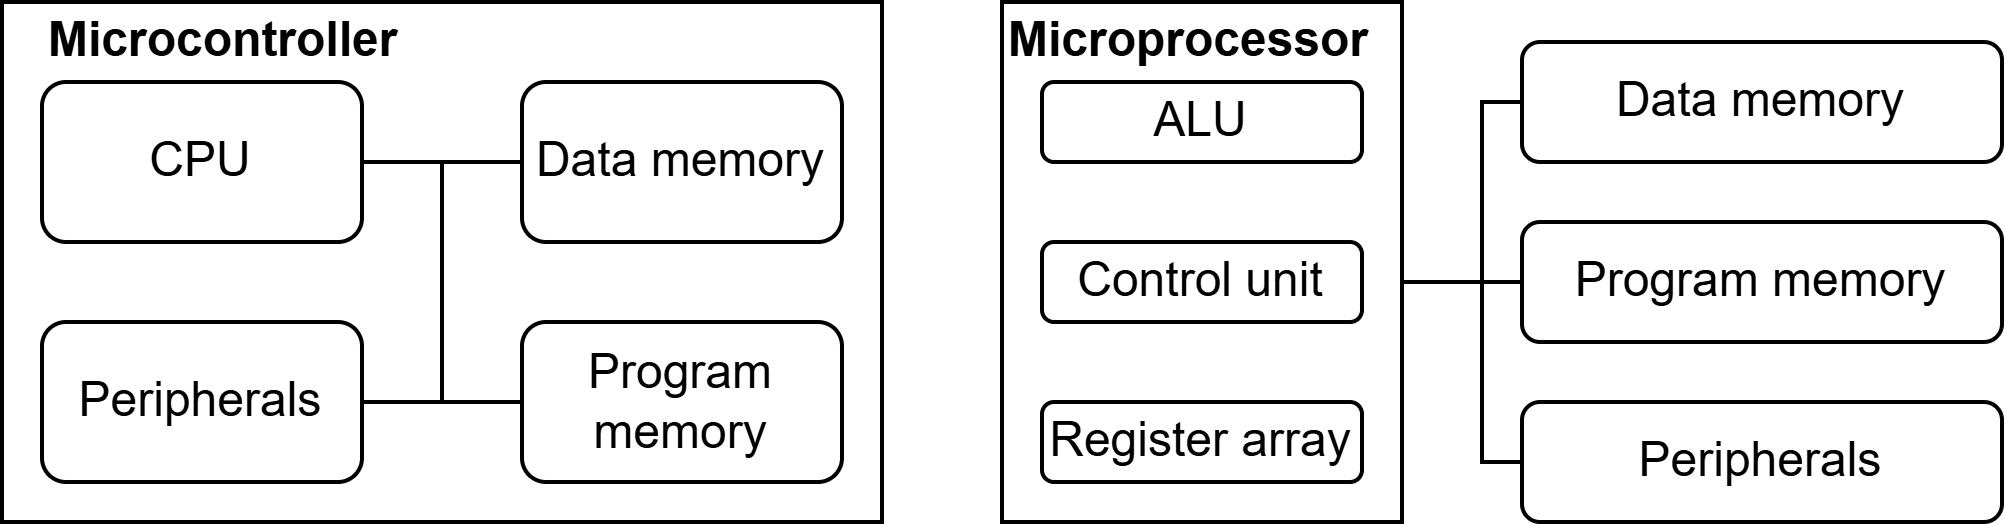
\includegraphics[width=0.75\linewidth]{images/eeai5.png}
    \caption{Microprocessor and microcontroller}
\end{figure}

\subsection{System on Chip}
A System on Chip (SoC) integrates all the core functionalities of a traditional computing system into a single chip.
This includes the CPU, memory, input and output interfaces, and sometimes specialized accelerators for AI, graphics, or signal processing.
They runs full operating systems and supports standard development tools and libraries. 
However, SoC have lower energy efficiency compared to microcontrollers, making them less ideal for ultra-low-power applications, and also more costly.